\documentclass[12pt,manuscript]{aastex}
\usepackage{savesym}
\savesymbol{tablenum}
\usepackage{siunitx}
\restoresymbol{SIX}{tablenum}
\usepackage{caption}
\usepackage{subcaption}
\usepackage{amsmath}
\usepackage{booktabs}
\usepackage{placeins}
 
\begin{document}

\newcommand{\Msun}{M_\odot}
\newcommand{\Lsun}{L_\odot}
\newcommand{\Rsun}{R_\odot}
\newcommand{\Mearth}{M_\oplus}
\newcommand{\Learth}{L_\oplus}
\newcommand{\Rearth}{R_\oplus}
\newcommand{\Mjup}{M_{Jup}}
 
\title{On the Relation Between Intrinsic and RV-Traced Exoplanet Observations}
\author{Cail Daley}
\altaffiltext{1}{Department of Astronomy and Van Vleck Observatory,
Wesleyan University, Middletown, CT, 06459; {\tt
cdaley@wesleyan.edu}}


\begin{abstract}
The true exoplanet distribution over a given parameter (planet mass, semi-major axis, etc.)  is not, of course, perfectly traced by the distribution derived from radial velocity (RV) observations. 
This is due to many factors and biases, in particular the bias towards high-mass planets close to their host star. 
Assuming these biases are well understood, it should be possible to find the “true” exoplanet distribution that corresponds to the distribution traced by RV techniques. 
While such a goal falls outsides the scope of this project, we take inspiration from this concept and explore the relations between intrinsic distributions and those traced by RV techniques.
Synthetic radial velocity curves are generated for an `intrinsic' distribution composed single-planet systems with a range of values for planet mass and orbital separation. 
The RV curves of nearly 6000 system are fit using a nested sampling algorithm, and an `observed' distribution is generated from these fits. 
This allows comparison between intrinsic and observed distributions, as traced by RV observations. 
Our results successfully reproduce relations inherent in the equations that determine radial velocity detection, as well as certain simple characteristics of the real-world exoplanet mass-orbital separation distribution.
\end{abstract}


%give keywords (see subject headings in http://dopey.mcmaster.ca/AASTeX/)
\keywords{methods: statistical, numerical --- techniques: radial velocities --- 
planets and satellites: detection, fundamental parameters}
\newpage

\FloatBarrier
\section{Introduction}
\label{section: intro}

Ever since the first positive discovery of an extrasolar planet by \cite{mayor95}, a major component of the study of exoplanets has been the detection, identification and characterization of individual exoplanets.
NASA's exoplanet archive lists 3558 confirmed exoplanets\footnote{https://exoplanetarchive.ipac.caltech.edu}, a large portion of which have been detected only in the past five years with the Kepler mission.
This sample has been built up with a wide variety of observational techniques, each sensitive to specific regions of the parameter space across which exoplanets are distributed. 
Some methods, like radial velocity or transit observations, are biased towards planets orbiting very close to their host star; others, like direct imaging, preferentially detect planets at large separations.

Exoplanets do not only serve as individual case studies---when taken as a whole, they constitute the observed exoplanet distribution.
Indeed, the observed incidence of certain subsets of the exoplanet population (super-Earths, hot Jupiters, etc.) has been used to constrain theories of planetary formation and migration, to name just two examples \citep{ida&lin04,boley16}.
However, a number of observational and instrumental effects introduce biases into our ability to detect exoplanets in certain regions of parameter space; the presence of such biases invites the conclusion that the exoplanet distribution implied by the sample of observed exoplanets is not the same as the true or intrinsic distribution.
While papers characterizing the observed exoplanet distribution are quite frank about this fact \citep[e.g.][]{marcy05,winn&fabrycky15}, exoplanetary astronomers often have no choice but to take reported incidence rates at face value, potentially propagating detection biases into other areas of the field.
As such, characterizing the intrinsic or true distribution of exoplanets as a function of fundamental parameters such as semi-major axis and mass is of vital importance to the field of exoplanets. 

 % the intrinsic distribution has been filtered through the biases specific to the various detection methods to produce the observed distribution. Indeed, we argue that for a given detection technique, we may think of the instrumental, observational, and statistical biases associated with that technique contributing to a mapping. This mapping transforms the intrinsic frequency distribution to an observed frequency distribution. It is dependent on a wide range of parameters (e.g. the planet eccentricity or the rotation rate of the host star) and may not have a functional form. Nevertheless, if the mapping for a given detection method can described (equivalent to the selection effects of the technique being well characterized), then it may be possible to recover information about the true exoplanet frequency distribution that is hidden in our observed distribution.


In the following pages, this concept is applied to the radial velocity detection technique. 
This involves: i) creating a synthetic `intrinsic' exoplanet distribution, ii) simulating a twenty-year radial velocity survey of the distribution, iii) fitting the observed RV curves with Bayesian statistical methods, and iv) compiling the fit information to create an observed distribution. 
This work certainly does not mark the first exploration of exoplanet populations using statistical methods; previous studies have generated exoplanet distributions using planet formation models \citep{ronco}, inferred the real-world intrinsic distribution from Kepler data by assuming a functional form for Kepler's detection efficiency \citep{traub16}, and
simulated and subsequently fit synthetic radial velocity curves in order to improve RV noise characterization \citep{dumusque16}.
Thus, in light of previous research this work falls somewhere between a proof-of-concept and a reproduction of already-understood biases inherent in the analytic equations that govern radial velocity detectability.
Because the biases that affect the intrinsic-to-observed mapping are myriad, it is not within the scope of this project to characterize them all accurately. 
This leads us to state one of the guiding principles of this project:
\textit{eliminate or mitigate the effect of all biases other than those we are interested in characterizing}.
This principle will be used throughout this work to justify various assumptions.

In Section \ref{section: distribution} the  distribution is described, and simplifying assumptions are justified.
Section \ref{section: survey} discusses the survey, and
Section \ref{section: fitting} details the fitting process.
In Section \ref{section: results} the resulting observed exoplanet distribution is presented and compared to the intrinsic distribution.
In Section \ref{section: conclusion} we summarize our results  and propose future work.
% The current state of the field is a product of countless hours of observations and analysis by both professional and amateur astronomers, and I would be remiss if I did not state my deep appreciation for their work.

% The true exoplanet distribution across a given parameter (planet mass, semi-major axis, etc.)  is not, of course, perfectly traced by the distribution derived from radial velocity observations. 
% This is due to a variety of factors and biases, e.g. the bias towards high-mass planets close to their host star. 
% Assuming we can accurately characterize these biases, it should be possible to find the “true” exoplanet distribution that corresponds to the distribution traced by RV techniques. 
% While such a goal falls outsides the scope of this project, I would like to take inspiration from this concept and explore the relations between intrinsic distributions and those traced by RV techniques. 
% This will be a primarily computational project, comprised of at least three major components: (i) creation of exoplanet distributions (ii) creation of an `observed' light curve for each planetary system in a distribution as part of a hypothetical RV survey, and (iii) fitting the lightcurve with MCMC (and possibly nested sampling) techniques. 
% Each component is discussed in a section below.
% As this project is still in its infancy in terms of implementation, I give a short description of my (planned) methodology and then mention some of the problems and questions I've been wrestling with in bullet points. I welcome all commentary, but the bullet points are the things I especially need help on.

\FloatBarrier
\section{The Distribution}
\label{section: distribution}

The distribution is comprised of almost 10,000 planetary systems; each system is defined by an inclination and a stellar mass. 
Each system is identical, with an inclination of \ang{90} and a stellar mass of \SI{1}{\Msun}.
Of course fixing the inclination at any value is not realistic,
but because inclination is a purely observational parameter unrelated to intrinsic exoplanet properties such as mass or semi-major axis, this decision will not introduce systematic biases into the synthetic distribution.
In addition, fixing the inclination at \ang{90} has the added bonus of making $m \sin i$ equivalent to $m$.
Fixing the stellar mass has two justifications.
Stellar mass is correlated with a host of other properties (for example, luminosity or spectral line contrast) that bias the real-world observed exoplanet distribution in a variety of ways. 
As we are not able to account for these effects, fixing the stellar mass is the best way to prevent unknown biases from slipping into our sample. 
Second, the majority of exoplanet systems detected by radial velocity lie around solar-mass stars (as seen in Figure \ref{fig: solar mass}), so fixing the stellar mass at \SI{1}{\Msun} allows better comparison between synthetic and real-world distributions.

\begin{figure}[ht]
  \centering
  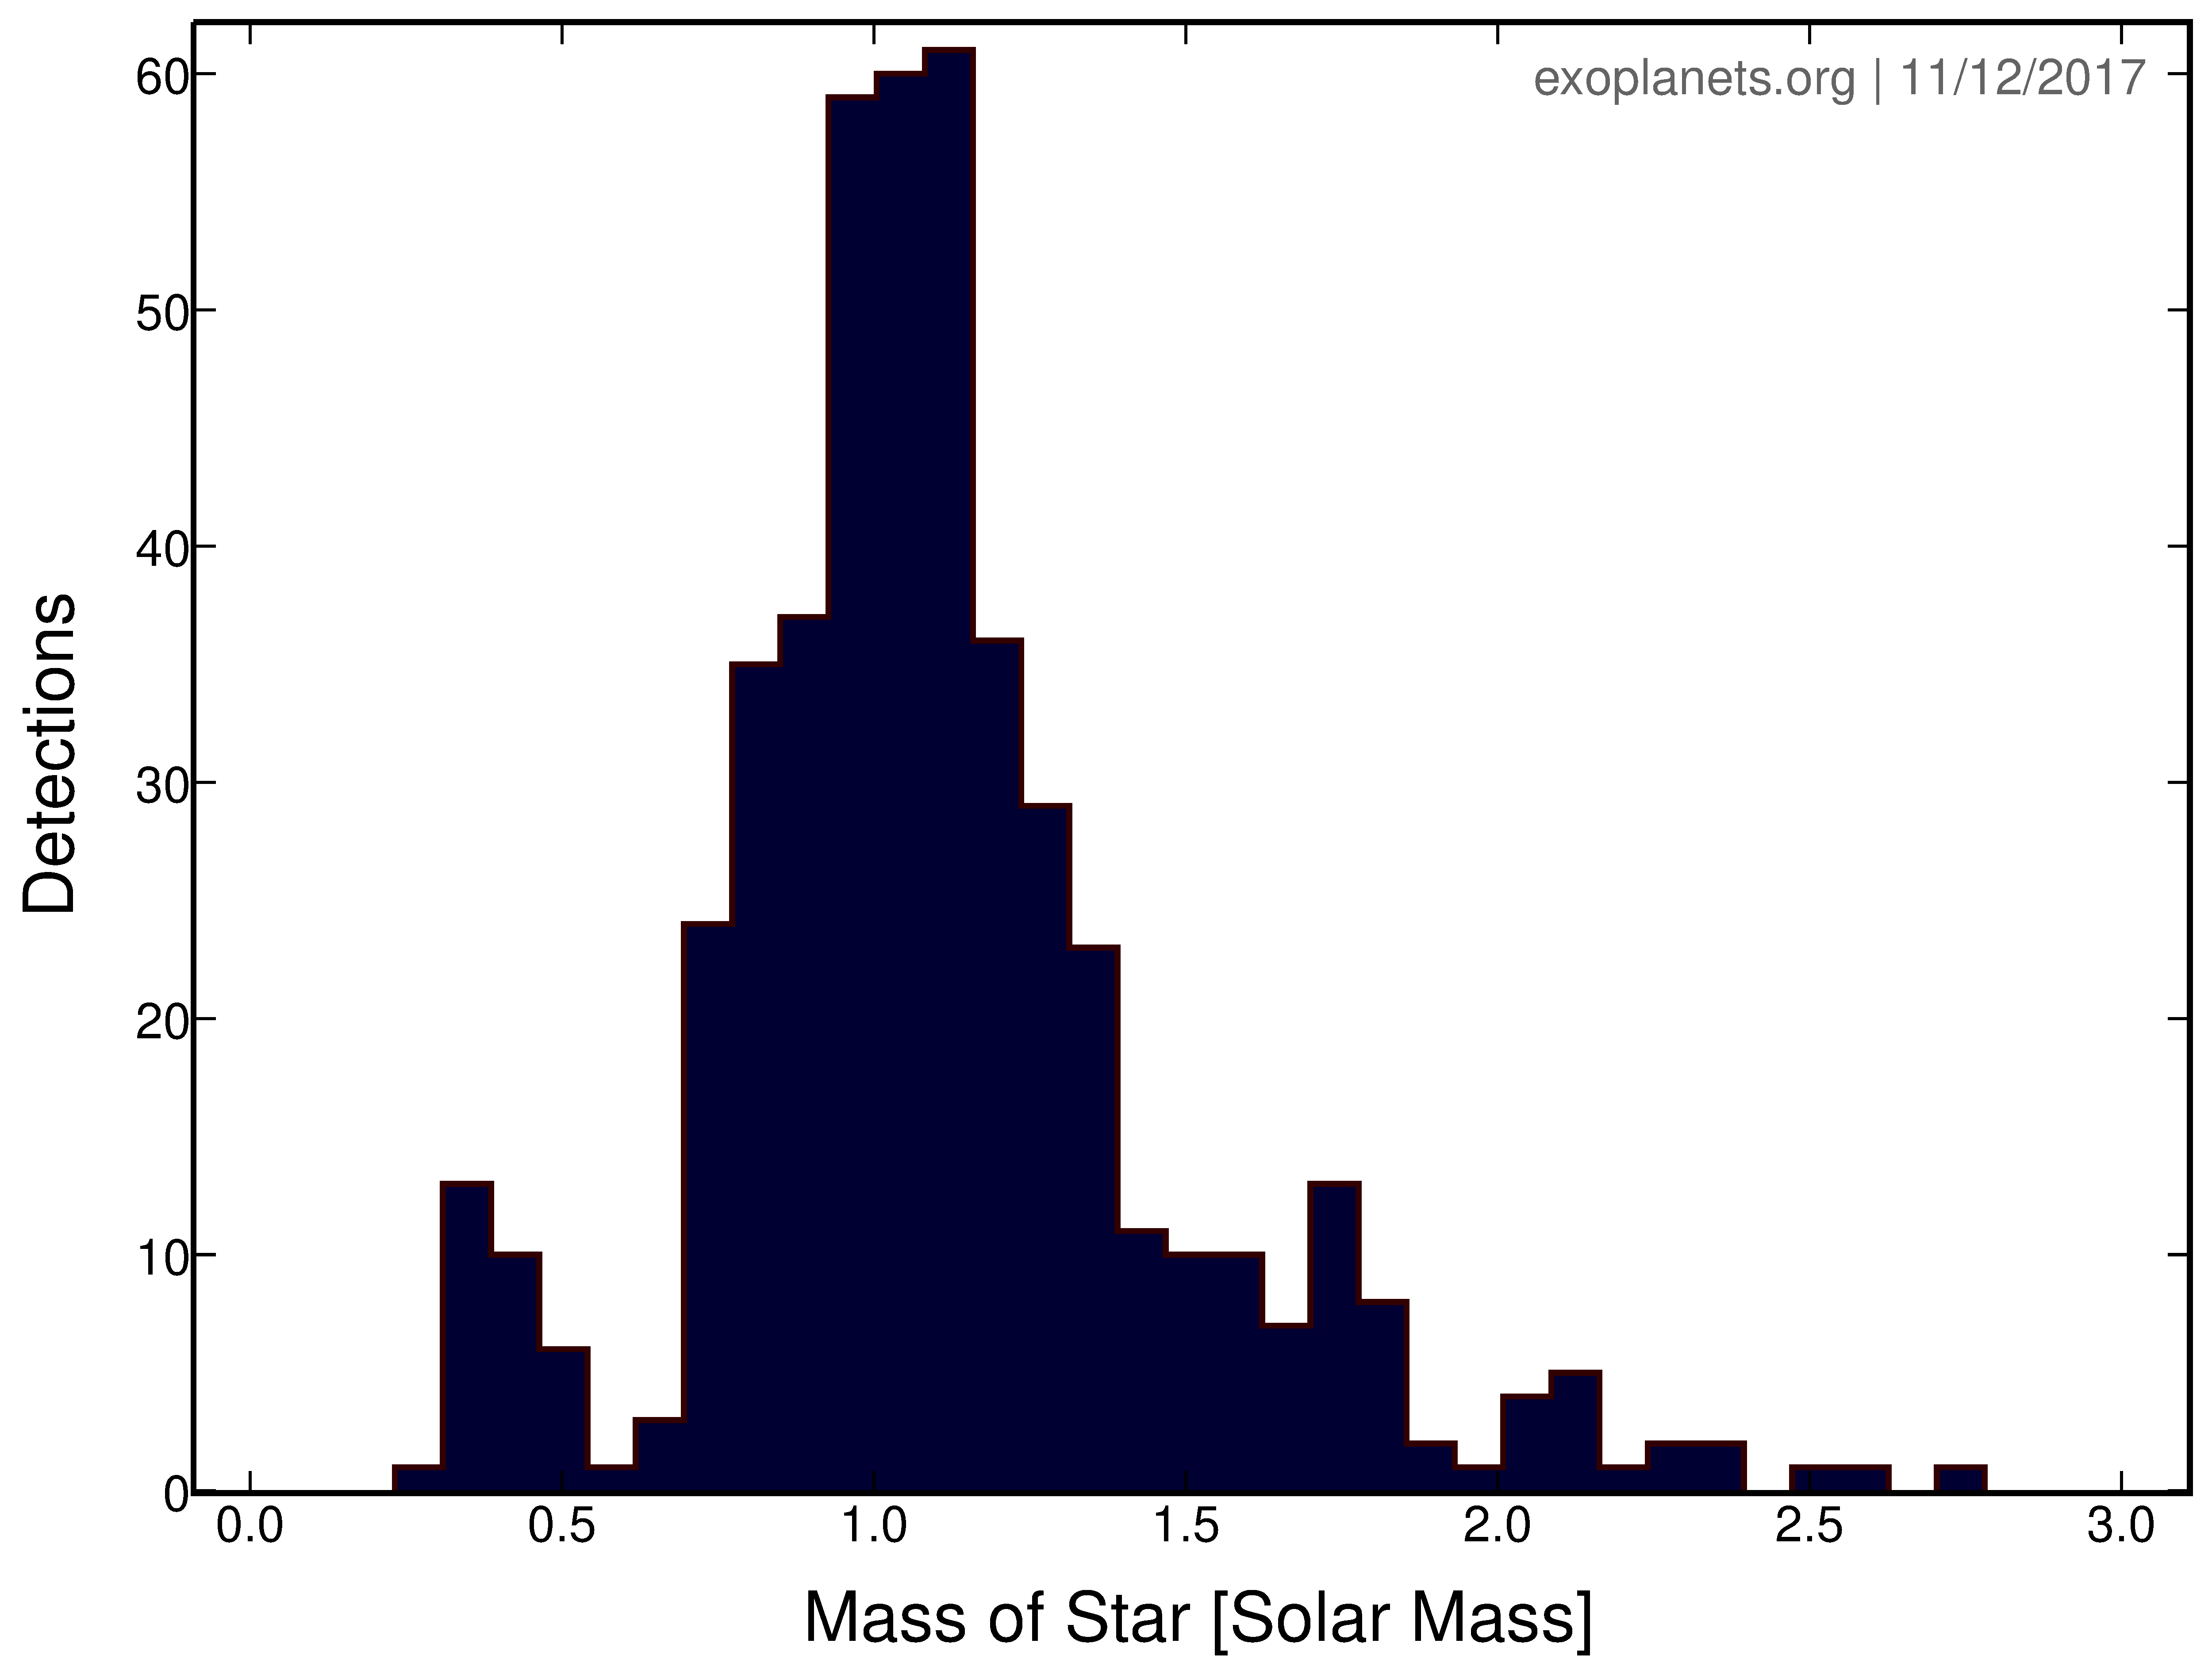
\includegraphics[width=0.5\linewidth]{../figures/solar_mass_detections}
  \caption{Number of radial velocity exoplanet system detections as a function of stellar mass.}
  \label{fig: solar mass}
\end{figure}

Each system is assigned exactly one planet. 
Planets are defined by a mass $m$, a semi-major axis $a$, an eccentricity $e$, an argument of periastron $\omega$, and time since periastron $t_0$. 
Eccentricity is set to zero for all planets; as $\omega$ is meaningless for $e=0$ it too is set to zero. 
The decision to fix eccentricity at zero was primarily motivated by difficulties in the fitting process. 
Exoplanet mass ranges between \SI{0.1}{\Mearth} and \SI{13}{\Mjup}, the brown dwarf mass limit. 
Semi-major axis ranges between \SI{0.1}{au} and \SI{10}{au}. 
This upper limit corresponds to a period of $\sim \SI{30}{yr}$, or 1.5 times the length of the survey discussed in the following section. 
As such, planets beyond \SI{10}{au} will have limited phase coverage, diminishing the confidence of detections.
Planets are spaced logarithmically between the boundaries given above, forming a two-dimensional logarithmic grid in $m-a$ parameter space. This allows easier comparison of the observed and intrinsic exoplanet distributions, as seen in Section \ref{section: results}.

\FloatBarrier
\section{Observations}
\label{section: survey}

Each exoplanet system is observed fifty times across the twenty year survey; the systemic radial velocity associated with a given date is calculated as follows. First, the mean anomaly $M$ is calculated from the planet's period $P$ and time since periastron passage $t_0$,
\begin{align}
  M = & 2\pi \frac{(t-t_0)}{P}.
  \intertext{The eccentric anomaly $E$ can be determined from $M$ by solving Kepler's Equation with a numerical solver:}
  M = & E - e \sin E 
  \intertext{and the true anomaly $f$ can be determined from $E$ as follows:}
  f = & 2\arctan \left( \sqrt{\frac{1 + e}{1 - e}} \frac{\sin E}{\cos E} \right).
  \intertext{Finally, the radial velocity of the star $v_{r,1}$ can be calculated now that $f$ is known:}
  v_{r,1} = & \sqrt{ \frac{G}{(m_1 + m_2)a(1-e^2)}} m_2 \sin i \\
  &\cdot (\cos(\omega + f) + e \cos \omega). \notag
\end{align}
This process is repeated for each date in the time series, generating a synthetic RV curve.
The resulting resulting curves agree well with theoretical predictions; for an $e=0$ Jupiter analogue around a solar analogue, a RV curve with $K_1 = \SI{28.42}{m/s}$ is produced, compared to the theoretical value of \SI{28.43}{m/s}.  
To make observations more realistic, Gaussian \SI{1}{m/s} noise is applied to produce the `observed' radial velocity curve.  We ignore all stellar noise contributions due to the difficulty in accurately characterizing them, and because of correlations between stellar noise and exoplanet characteristics (by way of spectral type, for example). 

\begin{figure}[ht]
  \centering
  \begin{subfigure}[b]{.9\linewidth}
    \centering
    \begin{tabular}{rcccc}
      \toprule
      Planet & $a$ (\si{au}) & $m$ (\si{\Mearth}) & $e$ & $P$ (\si{yr}) \\
      \midrule
      1 & 5.97 & 9.69 & 0.63 & 14.6 \\
      2 & 4.14 & 7.53 & 0.59 & 8.43 \\
      3 & 8.67 & 5.23 & 0.59 & 25.52 \\
      4 & 8.07 & 3.17 & 0.13 & 22.91 \\
      \bottomrule
    \end{tabular}
  \end{subfigure}
  
  \vspace*{1cm}
  
  \begin{subfigure}[b]{.75\linewidth}
  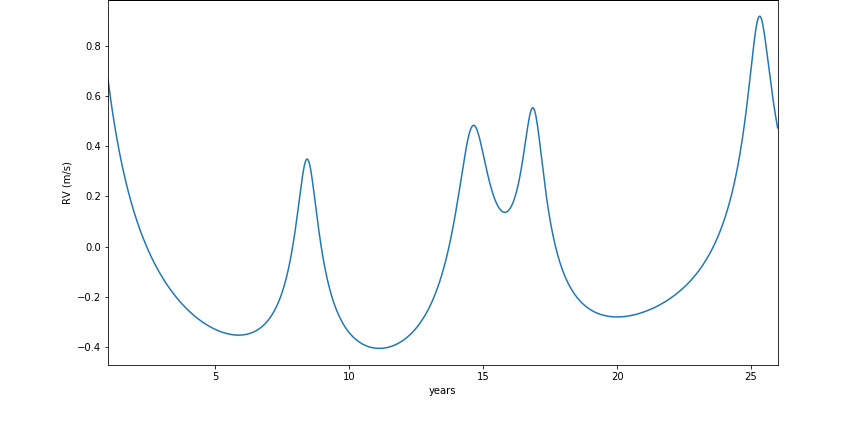
\includegraphics[width=\linewidth]{../figures/sample_curve}
  \end{subfigure}
  
  \begin{subfigure}[b]{.75\linewidth}
  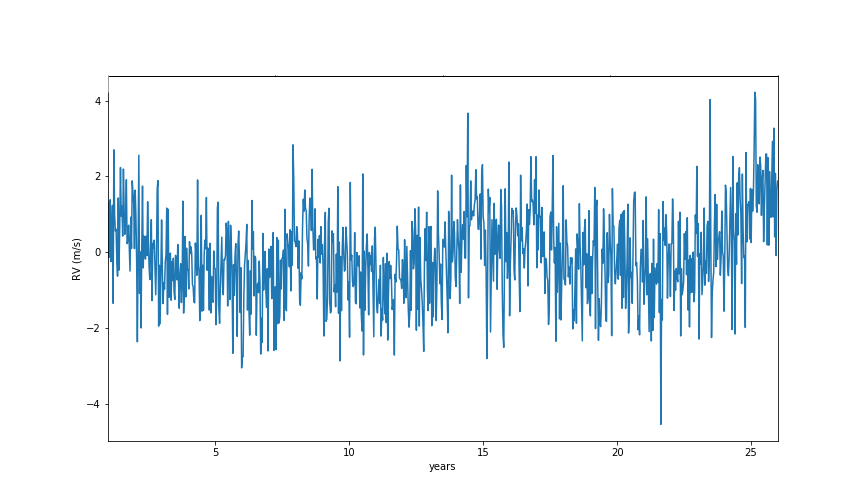
\includegraphics[width=\linewidth]{../figures/sample_curve_noisy}
  \end{subfigure}
  
  \caption{Top: Radial velocity curve of a four-planet system around a solar analogue, with planet parameters listed above. Bottom: The same system, but with \SI{1}{m/s} Gaussian noise added.}
  \label{fig: lightcurve}
\end{figure}


To produce self-consistent data that reasonably approximate real-world radial velocity observations, we assume that all of the synthetic observations are taken as part of the same radial velocity survey.
The survey is conducted over twenty years, with forty observations taken each night.
Imposing the requirement that each system is observed fifty times yields a exoplanet system size of $\sim 6000$ exoplanets. 
Observations are spaced logarithmically between \SI{1e5}{days} and $\num{1e5} + (20 \times \SI{365.25}{days})$ and then shifted back by \SI{1e5}{days}, so that the first observation occurs at $t=0$.
Because logarithmic spacing converges to linear spacing for very large numbers, this method results in almost-linearly spaced observations.
In fact, the observations are spaced such that the entire breadth of relevant frequency space is well sampled. 
Figure \ref{fig: periods} shows both the intrinsic and observed RV curves of two planets---one short-period and one long-period---as observed by the survey.
In both cases, coverage of the entirety of phase space is recovered.

\begin{figure}[ht]
  \centering
  
  \begin{subfigure}[b]{.45\linewidth}
  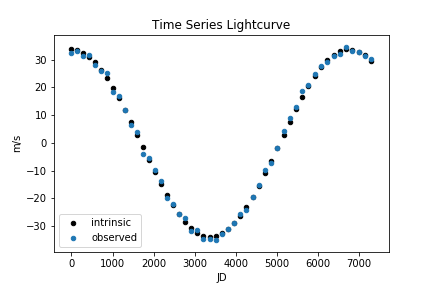
\includegraphics[width=\linewidth]{../figures/long_P_no_fold}
  \end{subfigure}
  \begin{subfigure}[b]{.45\linewidth}
  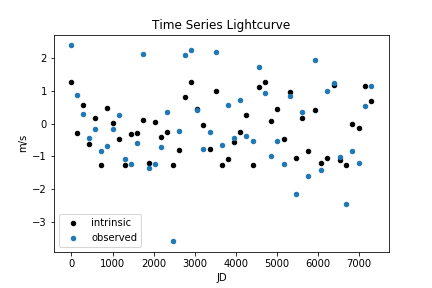
\includegraphics[width=\linewidth]{../figures/short_P_no_fold}
  \end{subfigure}
  
  
  \begin{subfigure}[b]{.45\linewidth}
  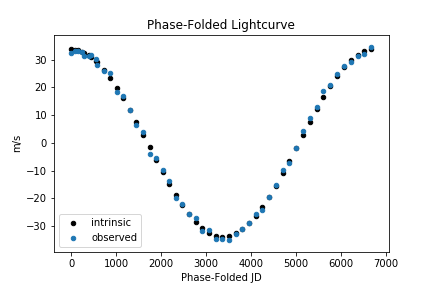
\includegraphics[width=\linewidth]{../figures/long_P_folded}
  \end{subfigure}
  \begin{subfigure}[b]{.45\linewidth}
  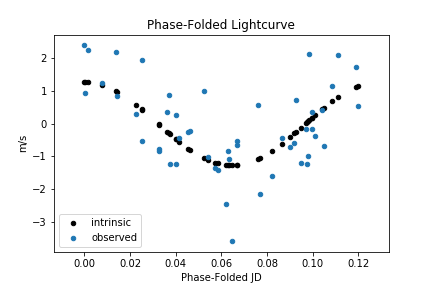
\includegraphics[width=\linewidth]{../figures/short_P_folded}
  \end{subfigure}

  \caption{The effect of logarithmic-almost-linear spacings between observations. On the left, the time series RV curve (above) and phase-folded RV curve (below) for a long-period exoplanet with $P \approx \SI{7000}{days}$ and $m = \SI{1000}{\Mearth}$. On the right, the same two plots for a short-period exoplanet with $P \approx \SI{0.12}{days}$ and $m=\SI{1}{\Mearth}$. In the phase-folded plots, the $x$-axis is in units of days rather than phase so as to show the large discrepancy in period between the two planets.  At both extremes, the entirety of phase space is well sampled.}
  \label{fig: periods}
\end{figure}



\FloatBarrier
\section{Fitting the Data}
\label{section: fitting}

The RV curve for each system is fit immediately after it is generated.
Due to a shortage of computation time, roughly one third of the planets in the system (all with $\log a < 0$) were not fit and are not included in the analysis.
Figure \ref{fig: 2d intrinsic} shows the regions of parameter space that were successfully fit.
Bayesian statistical techniques are used to `sample' parameter space and recover exoplanet properties; this is done by generating model radial velocity curves with different combinations of $m, a$ and $t_0$ ($e$ and $\omega$ are fixed to zero). 
The creation of these curves exactly follows the procedure described in Section \ref{section: survey}, except that noise is not added.
Model curves are then compared to the observed radial velocity curve and the log likelihood $L=-\chi^2/2$ is used to asses model quality of fit.
Thus log likelihood values are assigned to different combinations of $m$, $a$ and $t_0$, mapping out the log likelihood function throughout the three-dimensional parameter space.
In an ideal situation without noise, the log likelihood function in the neighborhood of the solution takes the form of a trivariate Gaussian centered at the solution.
Even with noise added, inspection reveals the log likelihood to be generally Gaussian.
This can be more intuitively understood if a two-dimensional parameter space is considered; here the parameter space is analogous to a topographic landscape, with regions of higher and lower likelihoods manifesting as peaks and troughs respectively.

The nested sampling fitting code \texttt{PyMultiNest}, a Python implementation of the Bayesian inference algorithm \texttt{MULTINEST}, is used to perform the sampling described above \citep{buchner14,feroz09}.
While an in-depth discussion of the \texttt{MULTINEST} algorithm falls outside the scope of this paper, a brief description is provded.
Nested sampling essentially calculates the model evidence $Z$ (the denominator of Bayes' Theorem) by transforming a $n$-dimensional integral over all of parameter space (i.e. the prior volume) to a one-dimensional sum across all likelihood values. 
This is accomplished by distributing a set of `live' points across parameter space. 
The point with the lowest-likelihood $L_0$ is iteratively removed from the set of live points and replaced with a new live point with likelihood $L > L_0$.
To increase efficiency, the new point is drawn from the volume enclosed by an $n$-dimensional ellipsoid generated from the covariance matrix of the live points that provides an estimate of the iso-likelihood contour given by $L=L_0$.
Thus the algorithm climbs through iso-likelihood contours that enclose decreasing volumes of parameter space until the remaining regions of parameter space are estimated to contribute an evidence $\Delta Z$ that is less than some predefined cutoff value. 
In this work, the iteration stops when $\log \Delta Z <0.5$.

As a final step, the evidence $Z$ is calculated by computing the `area under the curve' from the iso-likelihood contours via the trapezium rule.
The primary product of the nested sampling algorithm is, as described above, the evidence.
Because the evidence is the average likelihood over the prior parameter space, nested sampling allows parameter spaces defined by different hyperparameters (i.e. one planet vs. two planets) to be directly compared.
While different sets of model hyperparameters are not considered in this work, the current fitting structure could be expanded to include comparisons between models with different numbers of planets with relative ease.
Posterior probability distributions and the best-fit model can also be determined from the set of live and discarded points produced by nested sampling; we determine the `observed' exoplanet properties from the best-fit model parameters for each system.

Mass and semi-major axis are sampled logarithmically with uniform priors.
Logarithmic sampling was chosen to better cover the four and three orders of magnitude traversed by $m$ and $a$, respectively, and the prior volume is defined so that model planet properties remain physically justifiable.
Mass is confined to the range $\log(\SI{0.01}{\Mearth}) < \log m < \log (\SI{13}{\Mjup}) + 0.5$.
The overall bounds for semi-major axis are $\SI{0.05}{au} < a < \SI{11}{au}$; however setting a single prior for the semi-major axis proved difficult.
Because of the periodicity implicit in $a$ from Kepler's Third Law, for a given radial velocity curve there exists a family of `harmonics' of the correct solution.
For example, if a planet has a semi-major axis that corresponds to a period of \SI{2}{yr}, other solutions (more precisely, Gaussian local likelihood maxima in parameter space) exist at separations corresponding to periods of \SIlist[list-final-separator={, }] {0.5;1;4;6}{yr} and so on.
This is further complicated by the fact that due to the nonlinear relationship between separation and period ($a \propto P^{2/3}$), both the spacing and standard deviation of the Gaussian solutions diminish as $a_{true}$ decreases. 
From this we may conclude that fitting for $a$ becomes progressively harder as $a_{true} \to 0$ because the likelihood spike associated with the correct solution becomes more and more localized and thus harder for the algorithm to identify.

This effect is exacerbated by the logarithmic time spacing of observations described in Section \ref{section: survey}; as seen in Figure \ref{fig: periods}, for small $a_{true}$ consecutive observations do not trace consecutive points in the planet's orbital phase space but rather take snapshots of the radial velocity at ostensibly random, unordered points throughout phase space.
These effects combine to make the nested sampling algorithm systematically prefer higher values of $a$ in the regime $a_{true} \lesssim \SI{1}{au}$ as the harmonic solutions associated with larger $a$ tend to be broader and thus easier to find, even if they have lower log likelihoods.
As such, a decision tree was used to determine the prior in order to mitigate this effect.
If $a_{true} < \SI{2}{au}$, then the prior volume is defined such that $\SI{0.05}{au} < a < \SI{2.5}{au}$. 
On the other hand, if $a_{true} > \SI{2}{au}$ the prior is defined such that $\SI{1}{au} < a < \SI{11}{au}$. 
While this certainly not realistic---exoplanetologists will rarely know \textit{a priori} the correct regime for $a$---it is mostly a time-saving convenience rather than a necessary sacrifice. 
A more complex decision tree could be developed that determines the correct prior volume from a preliminary fit.
As such, we offer that this decision does not significantly affect the integrity of the project.

\begin{figure}[ht]
  \centering
  \begin{subfigure}[b]{.45\linewidth}
  \includegraphics[width=\linewidth]{../figures/{fit_SNR=0.5}.png}
  \end{subfigure}
  \begin{subfigure}[b]{.45\linewidth}
  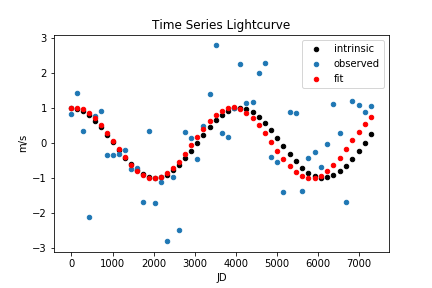
\includegraphics[width=\linewidth]{../figures/fit_SNR=1.png}
  \end{subfigure}
  \caption{Systems with model peak SNR of 0.5 (left) and 1 (right). While these examples are not necessarily representative of the entire sample, they do provide a sense of the limits of detection. The fit on the left is a non-detection, while the fit on the right lies at the lower end of the detection regime.}
  \label{fig: detection}
\end{figure}

Exoplanet detection is determined after the data has been fit. 
If the best-fit model peak signal-to-noise (SNR) ratio is greater than one, an exoplanet with said best-fit parameters is `detected;' the observed distribution is then generated from all such detections.
This cutoff was determined by trial and error. 
Best-fit models with peak SNR $< 1$ unreliably match the data, while those with peak SNR $> 1$ are in consistent agreement with the true values.
Figure \ref{fig: detection} shows examples of fits with model peak SNR above and below the detection limit.
While it may seem bizarre to use the \textit{model} peak SNR rather than the data peak SNR, two factors motivate this decision.
First, the peak SNR of the data is strongly affected by the Gaussian noise at the lower end of the detectability regime.
If detection was determined directly from the data SNR, the Gaussian noise would introduce a random component into detection algorithm.
Making use of the model peak SNR mitigates this random component, as the fitting does an excellent job of tracing the true, noiseless peak SNR.
As can be seen in Figure \ref{fig: 2d intrinsic}, the model SNR = 1 cutoff is remarkably consistent and also clearly illustrates the effect of mass and semi-major axis on the model SNR.
Indeed the model SNR = \numlist{1;10;100} cutoffs produced by this method agree very well with the \SIlist{1;10;100}{m/s} RV semi-amplitude isovelocity lines in $m$-$a$ space for a \SI{1}{\Msun} star, indicating that the model SNR successfully recovers the signal strength of the data \citep{ida&lin04}. 
Second, detection is determined before fitting even takes place if the data peak SNR is used.
This seems contrary to the philosophy of the project, which is driven by an interest in tracing the regime of exoplanet detectability as determined (in part) by fitting techniques.

\begin{figure}[ht]
  \centering
  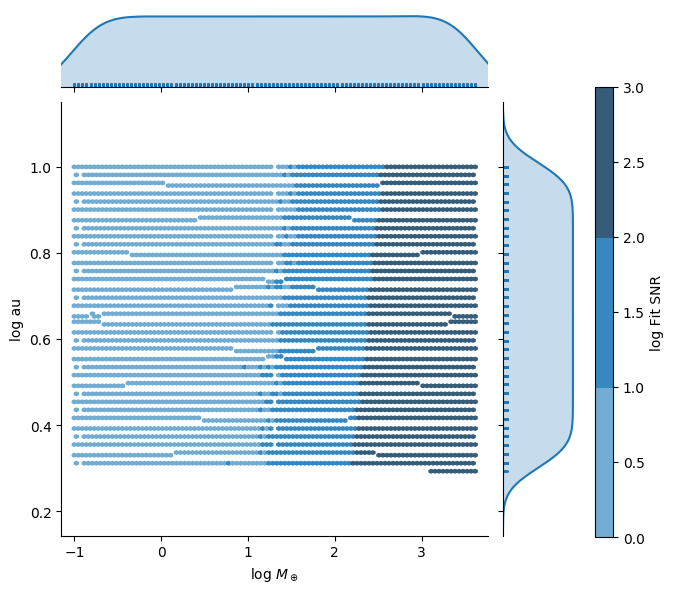
\includegraphics[width=.7\linewidth]{../figures/planets3_intrinsic}
  \caption{The intrinsic distribution sorted into hexagonal bins. Kernel density estimates (KDEs) of the one-dimensional mass and separation marginalized distributions are plotted along the edges. The KDEs are generated using a Gaussian kernel. The hexagonal bins are color-coded by the model log SNR; only systems with log SNR $>0$ are counted as detections.}
  \label{fig: 2d intrinsic}
\end{figure}


\FloatBarrier
\section{Results \& Discussion}
\label{section: results}

\begin{figure}[ht]
  \centering
  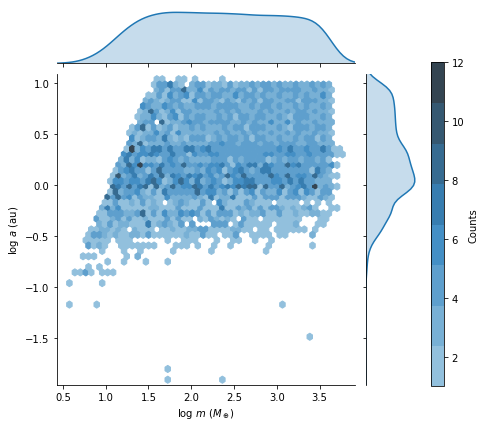
\includegraphics[width=0.7\linewidth]{../figures/planets3_observed}
  \caption{The observed distribution sorted into hexagonal bins. KDEs, generated in an identical manner to those of Figure \ref{fig: 2d intrinsic}, are plotted along the margins. The hexagonal bins are color-coded by the by number of systems in each bin; as such, the information represented encoded in the hue is different than in Figure \ref{fig: 2d intrinsic}.}
  \label{fig: 2d observed}
\end{figure}

Figure \ref{fig: 2d observed} shows the observed two-dimensional distribution of $m$ and $a$, the two exoplanet parameters of interest. 
The time since periastron $t_0$ is excluded from discussion in this section, as it is not a fundamental exoplanet property and does not exhibit notable correlations with either $m$ or $a$. 
The sharp cutoff imposed by the model SNR $ > 1$ detection condition can be clearly seen; the planet mass lower limit ranges from $\sim \SI{35}{\Mearth}$ at \SI{10}{au} to $\sim \SI{4}{\Mearth}$ at about \SI{0.1}{au}.
Additionally, a decrease in fit accuracy and consistency can be inferred as $m$ approaches the detection limit for a given $a$. 
For large values of $m$ and $a$, the observed exoplanet density remains largely constant, as evidenced by the consistent number of counts in each bin. 
% Indeed, because the fluctuation in the number of counts for massive planets seems to be patterned, we suggest that some of the fluctuation could be an artifact of misalignments between the hexagonal bin grid and the intrinsic exoplanet distribution grid.
In contrast, the count levels are much more chaotic at small $m$ and large $a$.
Some bins are empty (i.e. white) while others contain  up to seven exoplanets.
This indicates, unsurprisingly, that fitting becomes more difficult and less accurate as the SNR decreases.
It is difficult to assess the consistency of the fits in the low-$a$ regime, as the non-uniform nature of the intrinsic distribution cannot be easily separated from the consistency of the fits.

\begin{figure}[ht]
  \centering
  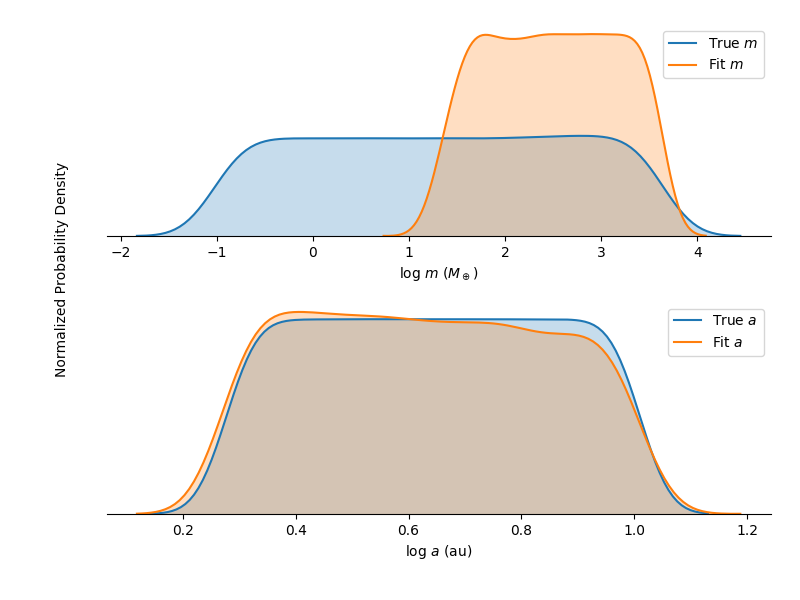
\includegraphics[width=0.9\linewidth]{../figures/planets3_comparison}
  \caption{Histograms of the intrinsic and observed density distributions of $m$ (top) and $a$ (bottom). Histogram bin sizes are chosen such that the bin size is equal to the spacing of the intrinsic distribution.}
  \label{fig: comparison hist}
\end{figure}

Figure \ref{fig: comparison hist} shows a comparison of the intrinsic and observed distributions for $m$ and $a$.
In keeping with Figure \ref{fig: 2d observed}, a bias towards large masses is apparent, as well as a very slight downward trend in the detection fraction with increasing $a$ (at least for $0 < \log a < 1$).
Although the sparse and inconsistent coverage for $a < 0$ makes it difficult to make statements about the detection fraction in this regime, we note with caution that the detection actually seems to \textit{decrease} as $a\to 0$.
This runs contrary to the relations given by the analytic equation for radial velocity semi-amplitude; one would expect the signal, and thus the detection fraction, to increase as $a \to 0$.
We suggest this analytic bias towards small separations is overwhelmed by the fitting algorithm bias against separations described in Section \ref{section: fitting}, causing a net decrease in the detection fraction as  $a \to 0$.

\begin{figure}[ht]
  \centering
  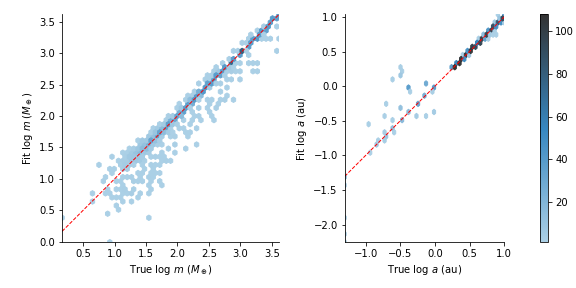
\includegraphics[width=0.9\linewidth]{../figures/planets3_correlations}
  \caption{Two-dimensional histograms showing the correlations between intrinsic and observed distributions for both mass and semi-major axis. 
  Hue once again denotes the number of exoplanets falling into each hexagonal bin.
  The red dashed lines trace a one-to-one correspondence between observed and intrinsic properties; thus, the scatter around the red dashed lines shows the accuracy the fitting.}
  \label{fig: correlations}
\end{figure}


Further evidence for this hypothesis is provided in the right-hand pane of Figure \ref{fig: correlations}, which shows the correlations between the intrinsic and observed properties for the distribution.
A perfect fit would result in $a_{true} = a_{fit}$, so any deviation from a one-to-one correspondence  between intrinsic and observed values (traced by the red dashed line) indicates an inaccurate fit.
The scatter around the red line remains small for $\log a \gtrsim 0$, indicating that the fits are consistent with the true values in this region. 
However, for $\log a \lesssim 0$ $a_{fit}$ is systematically larger than $a_{true}$.
As the fitting bias described in Section \ref{section: fitting} increases the chances of the fitting algorithm converging to a `harmonic' of the true solution associated with larger $a$, one would expect the fits to overestimate $a$ at small separations.
We expect to see a symmetric effect in the mass correlation plot of Figure \ref{fig: correlations}, as increasing the fit orbital separation in turns requires an increase in planet mass to keep the model signal on the same level as the signal in the data.
However, the opposite effect seems to occur: the fitting systematically underfits the data.
The cause of this underfitting is unclear.
Also of interest in the mass correlation plot is the increasing scatter as $m$ decreases; we interpret this as the result of the decreasing $SNR$ of the data in this regime.

\begin{figure}[ht]
  \centering
  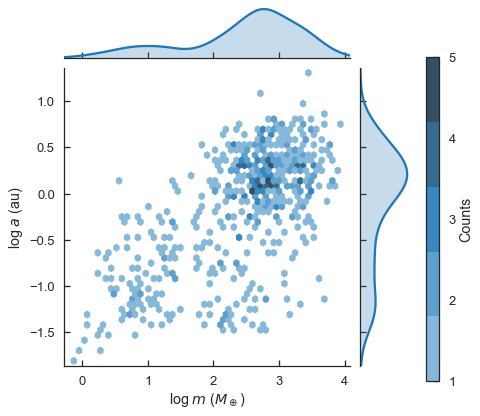
\includegraphics[width=0.7\linewidth]{../figures/real_world_dist}
  \caption{The `real-world' $m-a$ distribution of radial velocity-detected exoplanets, sorted into hexagonal bins. KDEs are plotted along the margins, and the hexagonal bins are color-coded by the by number of systems in each bin.}
  \label{fig: 2d real world}
\end{figure}

As a final step, the `observed' exoplanet distribution generated by the fitting pipeline is compared to the `real-world' distribution of radial velocity-detected exoplanets.
The high $a$/low $m$ region is unpopulated in both plots, as expected---current radial velocity techniques lack the sensitivity to detect planets in this regime, regardless of the underlying distribution.
Surprisingly, while the mass lower limit compares well between observed and real-world distributions for small $a$ ($\log m \approx 0.75$ at $\log a \approx -0.5$ for both distributions) the lower limits diverge by about an order of magnitude at large $a$ ($\log m \approx 1.5$ for the observed distribution compared to $\log m \approx 2.5$ for the real-world distribution at $\log a \approx 1$).
While this is only a rough estimate, such a large discrepancy between the mass lower limit slopes might suggest the existence of detection biases in the real-world distribution beyond those inherent in the analytic radial velocity equations.
We are hesitant to draw any further correlations between observed and real-world distributions due to the large number of biases in the real-world sample that we do not characterize.

\FloatBarrier
\section{Conclusions}
\label{section: conclusion}

This work has attempted to characterize a small fraction of the biases associated with radial velocity detection techniques, namely those inherent in the equations that govern the strength of radial velocity signals, in order to understand and predict the relations between intrinsic and observed distributions.
A uniform `intrinsic' exoplanet distribution was generated and each exoplanet system in the distribution was subsequently fit with a nested sampling algorithm, yielding an `observed' distribution of exoplanet masses and orbital separations.
Due to the large number of simplifying assumptions made, the results reveal only the most common-sense aspects of the intrinsic-to-observed mapping.
Comparison between observed and real-world distributions was also hindered by a bias against small orbital separations that was introduced into the fitting pipeline by certain characteristics of the likelihood function as well as by peculiarities in the spacings between data points used to generate RV curves.
Nevertheless, the negligible detection fraction in the high-$a$ low-$m$ regime does allow us to conclude that the sparsity of real-world exoplanet detections in this area is most likely a function of sensitivity limitations rather than an underdensity in the underlying population.
This does not, however, preclude such an underdensity from existing.
Additionally, a linear decrease in the minimum-mass detection limit with increasing orbital separation is observed in both the real-world and synthetic observed distributions, although the slopes of these limits differ significantly.

Further work could improve this project in a number of ways.
Multi-planet systems could be introduced, as well as planets with non-zero eccentricities and arguments of periastron. 
Stellar spectral type and metallicity could also be included.
A more accurate model of radial velocity noise could be developed, taking into account stellar and instrumental noise sources \citep[e.g.][]{dumusque16}.
A non uniform distribution could also be implemented, allowing better comparison between the real-world distribution and the observed distribution.
Indeed, with rigorous characterization of radial velocity detection biases it may be possible to fit the synthetic observed distribution to the observed real-world distribution, allowing statements to be made about the intrinsic real-world exoplanet distribution.

\begin{thebibliography}{}

\bibitem[Boley et al.(2016)]{boley16} Boley, A.~C., Granados Contreras, A.~P., \& Gladman, B.\ 2016, \apjl, 817, L17 

\bibitem[Buchner et al.(2014)]{buchner14} Buchner, J., Georgakakis, A., Nandra, K., et al.\ 2014, \aap, 564, A125

\bibitem[Dumusque(2016)]{dumusque16} Dumusque, X.\ 2016, \aap, 593, A5 

\bibitem[Feroz et al.(2009)]{feroz09} Feroz, F., Hobson, M.~P., \& Bridges, M.\ 2009, \mnras, 398, 1601 

\bibitem[Ida \& Lin(2004)]{ida&lin04} Ida, S., \& Lin, D.~N.~C.\ 2004, \apj, 604, 388 

\bibitem[Marcy et al.(2005)]{marcy05} Marcy, G., Butler, R.~P., Fischer, D., et al.\ 2005, Progress of Theoretical Physics Supplement, 158, 24

\bibitem[Mayor \& Queloz(1995)]{mayor95} Mayor, M., \& Queloz, D.\ 1995, \nat, 378, 355 

\bibitem[Ronco et al.(2017)]{ronco} Ronco, M.~P., Guilera, O.~M., \& de El{\'{\i}}a, G.~C.\ 2017, \mnras, 471, 2753 

\bibitem[Traub(2016)]{traub16} Traub, W.~A.\ 2016, arXiv:1605.02255 

\bibitem[Winn \& Fabrycky(2015)]{winn&fabrycky15} Winn, J.~N., \& Fabrycky, D.~C.\ 2015, \araa, 53, 409 

\end{thebibliography}

 \end{document}
